 \begin{tikzpicture}[imgstyle/.style={draw,thick,anchor=south west,inner sep=1pt}]
 %\path[use as bounding box, draw] (0,-1) rectangle (\imgwidth, 0.34\imgwidth);
\node[imgstyle] (img1) at (0,0) {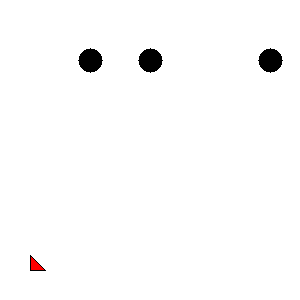
\includegraphics[width=0.32\imgwidth]{media/frame0000.png}};
\node[imgstyle] (img2) at (0.333\imgwidth,0) {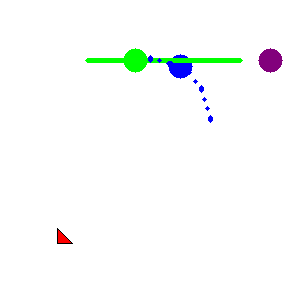
\includegraphics[width=0.32\imgwidth]
{media/frame0003.png}};
\node[imgstyle] (img3) at (0.666\imgwidth,0) {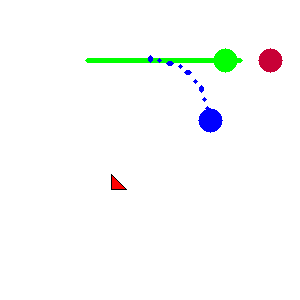
\includegraphics[width=0.32\imgwidth]{media/frame0009.png}};
\begin{scope}[x={(img1.south east)}, y={(img1.north west)}]
\node (r) at (0.3, 0.1) {Robot};
\node (lmks) at (0.7, 0.6) {Landmarks};
\node (t1) at (0.9, 0.1) {t=0};
\end{scope}
\begin{scope}[x={(img2.south east)}, y={(img2.north west)}]
\node (t1) at (0.9, 0.1) {t=3};
\end{scope}
\begin{scope}[x={(img3.south east)}, y={(img3.north west)}]
\node (t1) at (0.9, 0.1) {t=9};
\end{scope}
\path ($(img1.south) + (-0.5, -0.5)$) node (ld) {Legend:};
\path 
(ld)
 ++ (1.8, 0) node [circle,fill=green] {} + (1, 0) node {Prismatic}
 ++ (3, 0) node [circle,fill=blue] {} + (1, 0) node {Revolute}
 ++ (3, 0) node [circle,fill=red] {} + (0.8, 0) node {Static}
;

 \end{tikzpicture}
